\documentclass{report}
\usepackage{contour}
\usepackage{ulem}
\usepackage{caption}
\usepackage{subcaption}
\usepackage{geometry}
\geometry{
letterpaper,
left=1in,
right=1in,
bottom=1in,
top=1in,
}

\renewcommand{\ULdepth}{1.5
pt}
\contourlength{0.8pt}

\newcommand{\myuline}[1]{%
  \uline{\phantom{#1}}%
  \llap{\contour{white}{#1}}%
}

\renewcommand{\baselinestretch}{1.5}

\begin{document}

\begin{titlepage}
    \begin{center}
        \vspace*{1cm}
 
        \textbf{MSE160S Microstructure-Property Relationship Final Report}
 
        \vspace{0.5cm}
        \textit{Designing a Polymer for "Hinged" Compliant Mechanisms}
             
        \vspace{1.5cm}
 
        J. Lefebvre\\\small{jayden.lefebvre@mail.utoronto.ca}\\\small{Student Number: 1006861344}
 
        \vfill
             
        \vspace{0.8cm}
             
        Engineering Science\\
        Faculty of Applied Science and Engineering\\
        University of Toronto\\
        Tuesday April 27th, 2021
             
    \end{center}
 \end{titlepage}

% \maketitle

\section{Introduction}

Compliant mechanisms are a category of simple mechanical devices used to transform force and motion via \textbf{elastic deformation and deflection}.
They have become increasingly popular as an alternative to more traditional rigid and jointed systems for a variety of reasons, dependent on the use case \cite{compliant}.
Their potential use cases are immensely broad, ranging from sensitive surgical instrumentation (that must respond and react to subtle muscle movements and deflect so as to not cause tissue damage) to emergency safety mechanisms designed to prevent the accidental firing of nuclear weapons \cite{invention}.
Although typically made from \textbf{plastics} and other polymers, they may also be made from ductile metals (or even paper in the case of "action origami", which I think is pretty neat) \cite{invention}. For the purposes of this report, only plastics will be considered.
\vspace{1cm}

\begin{figure}[h]
    \label{fig:wrench}
    \centering
    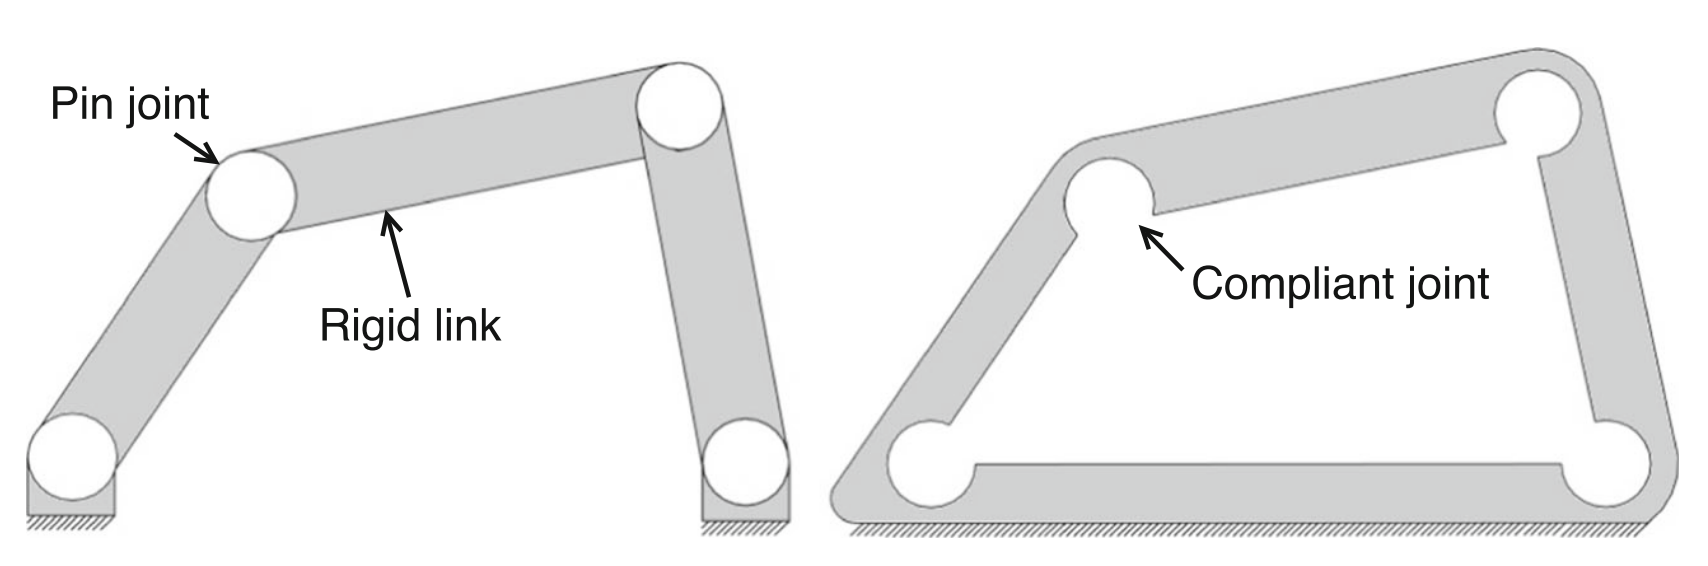
\includegraphics[width=\textwidth]{images/comparison.png}
    \hfill
    \caption{Two equivalent mechanisms: a typical rigid, jointed mechanism (left) and a compliant, bending mechanism (right) \cite{functionallygradedmaterials}.}
\end{figure}

One of the simplest and most common compliant implementations is in "hinge" components (those transferring work solely rotationally). Bending about a main axis is central to the operation of these mechanisms.
Where traditional hardware mechanisms have pin joints (pins fastening two or more bodies about which they freely rotate), compliant mechanisms \textbf{bend} at specific locations with thinner cross-sectional area relative to the bending moment, known as "compliant joints" \cite{compliant}. 

\pagebreak
\section{Hinge Fatigue via Repetitive Stress}

Just as any typical hardware mechanism must be designed to withstand many, \textit{many} uses (often on the order of hundreds of thousands, or more), compliant mechanisms aiming to solve similar problems 
must be designed to "comply" just as many times \cite{rotationalhinges}. However, where traditional hardware mechanisms experience very gradual (often unnoticeable) surface wear as a result of \textit{sliding friction} within the joints, compliant mechanisms experience permanent deformation over time
as a result of \textbf{repeated \textit{elastic} stress} within the bending compliant joint. 
\vspace{1cm}
\begin{figure}[h]
    \label{fig:latch}
    \centering
    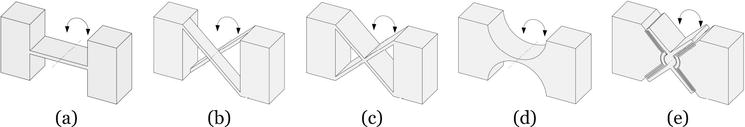
\includegraphics[width=\textwidth]{images/hingetypes.png}
    \hfill
    \caption{A variety of compliant hinge topologies \cite{hingedesign}.}
\end{figure}

The flexural stress $\sigma$ experienced by the joint (and hence, the deflection) is proportionate to the bending moment at that loaction, and inversely proportionate to the second moment of area $I$ of the joint at that location, and thus the cross-sectional area.

\begin{equation}
    \sigma (x) \propto \frac {M(x)}{I(x)}
\end{equation}

Although specific topologies and designs of hinges is outside of the realm of microstructure-property relationships, it is important to consider the role of cross-sectional area to the \textbf{origin and propagation} of elastic flexural-stress-induced fatigue: 
where the material is thin (i.e. where it is intended to bend, at the intended joint), it experiences a greater stress than other locations.

\section{Microstructure: Fatigue Origins and Parameters}

In order to speak properly about the specifics of fatigue at the microstructure level, we must first accurately define it: "Polymer fatigue is the process of damage to the friction surface of polymer caused by repeated cyclic stresses (deformations) whose amplitude does not exceed the ultimate strength of the polymer." \cite{Bogdanovich2013}

\begin{figure}[h]
    \label{fig:latch}
    \centering
    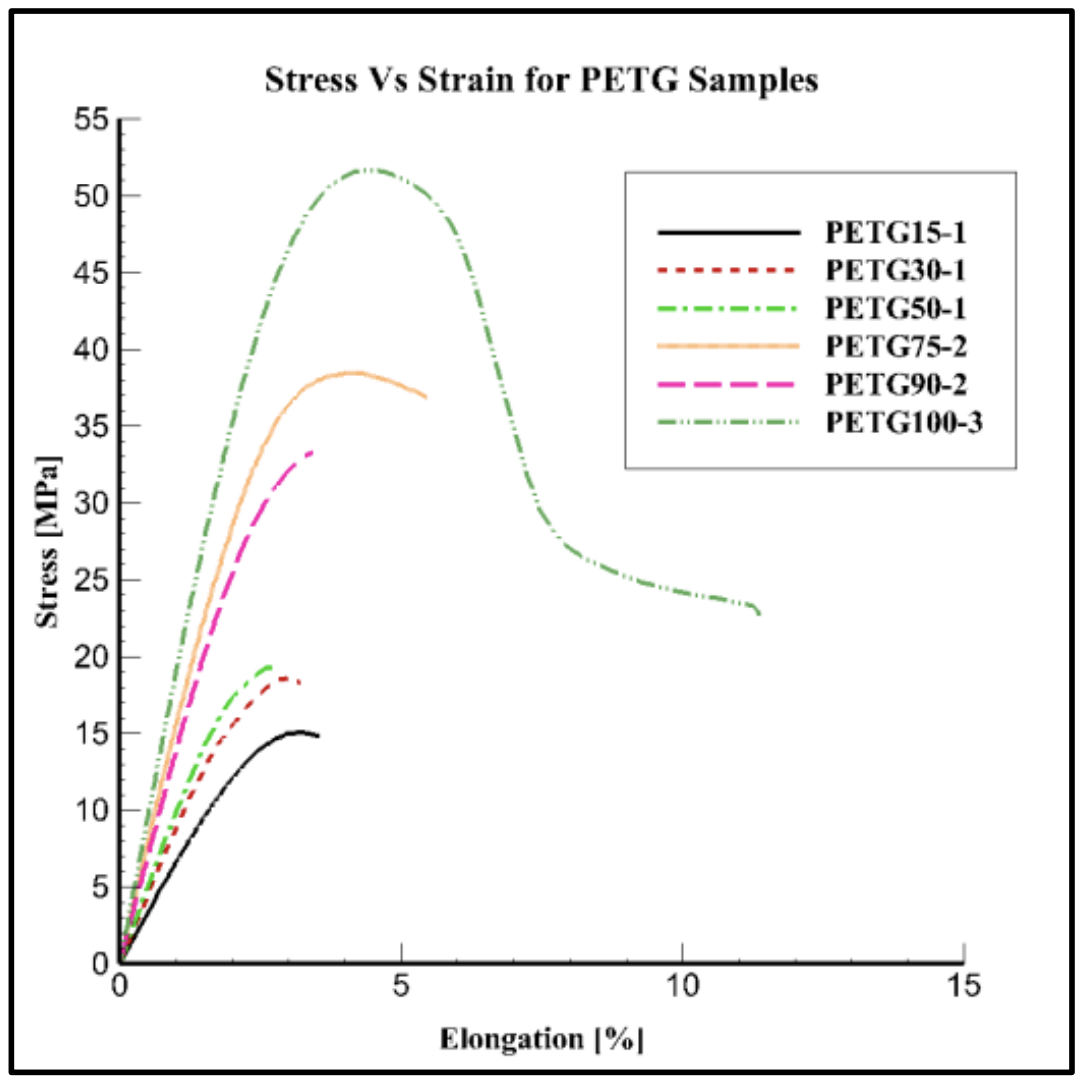
\includegraphics[width=\textwidth/2]{images/stressstrain.png}
    \hfill
    \caption{Stress vs strain curve for PETG samples of various levels of "infill" (additive manufacturing density) \cite{infill}.}
\end{figure}

Invisible to the naked eye, under repetitive elastic deformation, "faults are introduced at the molecular level ... After many deformations, cracks will begin to appear, followed soon after by a fracture, with no apparent plastic deformation in between" \cite{fatigue}.
The fatigue process begins with dislocation movements, which eventually form \textbf{persistent slip bands} (PSBs) that ultimately become the origin of larger-order failure.

% \begin{figure}[h]
%     \label{fig:latch}
%     \centering
%     \begin{subfigure}[b]{0.48\textwidth}
%         \centering
%         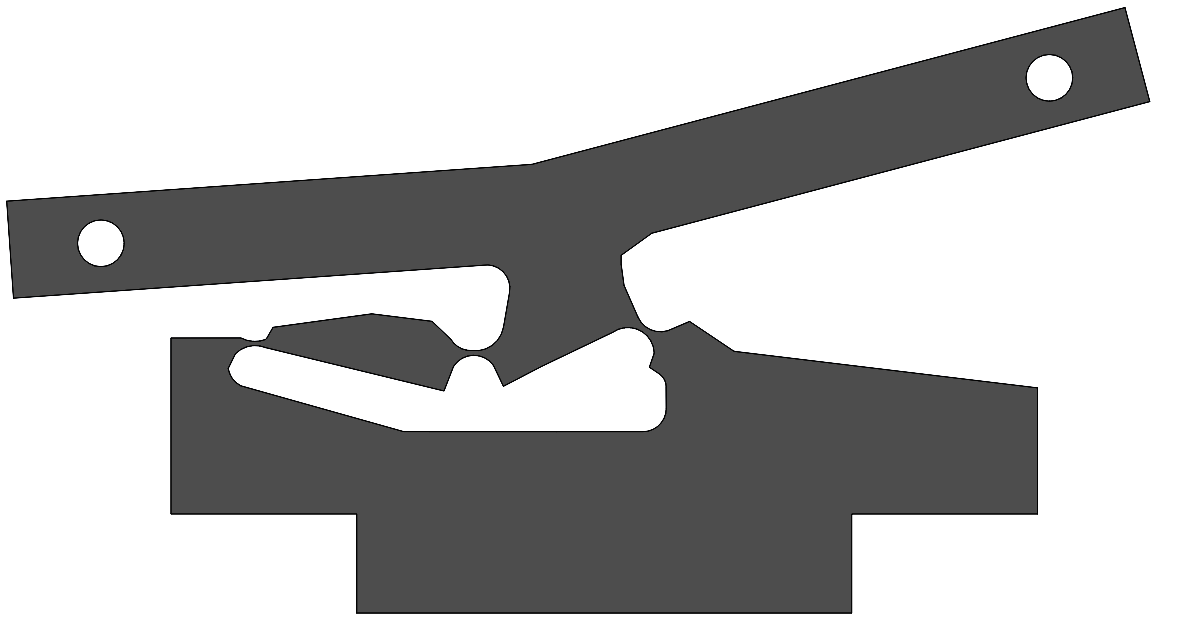
\includegraphics[width=\textwidth-1cm]{images/latchl.png}
%     \end{subfigure}
%     \hfill
%     \begin{subfigure}[b]{0.48\textwidth}
%         \centering
%         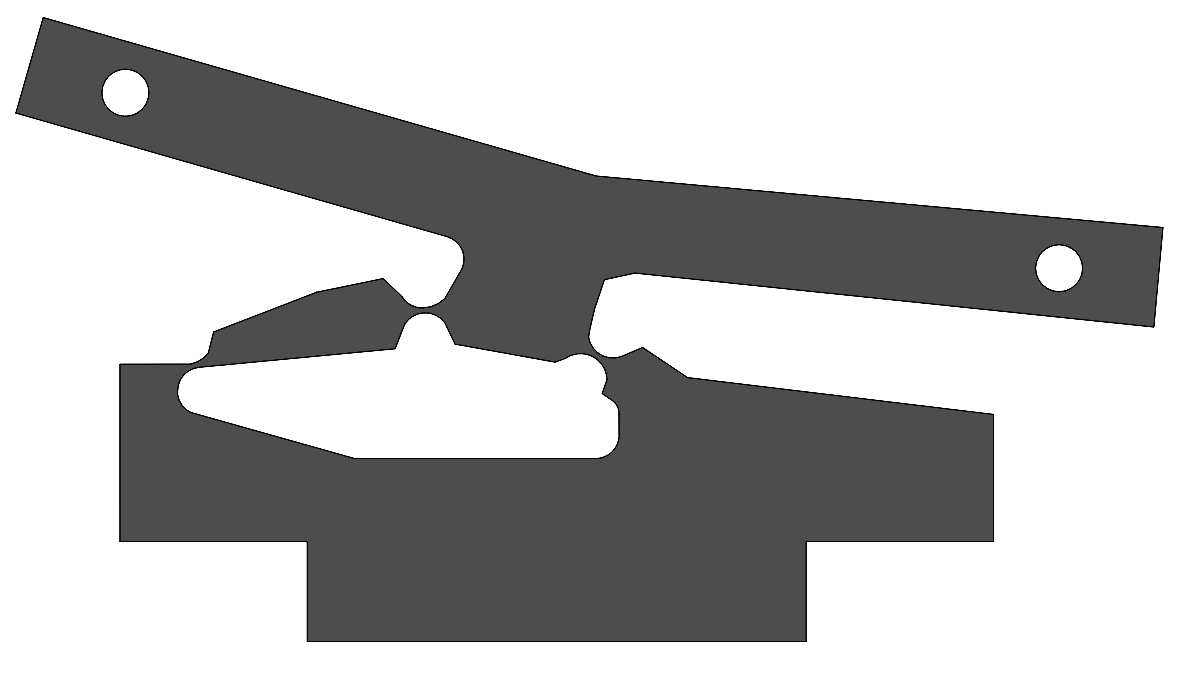
\includegraphics[width=\textwidth]{images/latchr.png}
%     \end{subfigure}
%     \hfill
%     \caption{A pair of compliant hinges forming a latch (or switch), shown here in its two possible positions \cite{wiki}.}
% \end{figure}

Fatigue life (number of cycles before fatigue) is influenced by a variety of factors, including environment (temperature, humidity, etc.), surface finish, metallurgical microstructure, presence of oxidizing or inert chemicals, residual stresses, and (most importantly) the magnitude of the repetitively applied stress (proximity to the plastic region). 
Unfortunately, the fatigue process is also (to a degree) random, often displaying considerable scatter even in seemingly identical samples in well controlled environments \cite{fatigue}.

\section{Conclusion}

In order for critical compliant mechanisms to be reliable over long lifetimes, they must be made of materials resilient to high-cycle fatigue. Polymers intended for these applications must be resistent to dislocation movements while maintaining suitable flexibility AND stiffness for the design application (with a specific focus on "hinges").

\pagebreak
\section{References}

\bibliographystyle{IEEEtran}

\bibliography{references}

\end{document}